%% Based on a TeXnicCenter-Template by Gyorgy SZEIDL.
%%%%%%%%%%%%%%%%%%%%%%%%%%%%%%%%%%%%%%%%%%%%%%%%%%%%%%%%%%%%%

%----------------------------------------------------------
\documentclass{report}%
\usepackage{amsmath}%
\usepackage{amsfonts}%
\usepackage{amssymb}%
\usepackage{graphicx}
\usepackage[T2A]{fontenc}
\usepackage[utf8x]{inputenc}
\usepackage[english, russian]{babel}
%----------------------------------------------------------
\newtheorem{theorem}{Теорема}
\newtheorem{claim}{Утверждение}
\newtheorem{definition}{Определение}
\newtheorem{lemma}{Лемма}
\newtheorem{remark}{Замечание}
\newenvironment{proof}{\par\noindent{\bf Доказательство.}}{\hfill$\scriptstyle\blacksquare$}
%----------------------------------------------------------
\begin{document}
\frenchspacing
%\numberwithin{equation}{chapter}
\binoppenalty=10000
\relpenalty=10000
\setcounter{secnumdepth}{-1}
\title{Хроматические числа}
\author{Гольцова Надежда}
\date{\today}
\maketitle

\section{Обзор результатов}

Задача о нахождении хроматического числа плоскости была поставлена             
Э.~Нелсоном в 1950~г. и~остается не~решенной до сих пор. Её формулировка: 
какое наименьшее число цветов необходимо для такой раскраски плоскости, 
при~которой любые две точки на~расстоянии~1 друг от~друга покрашены в~разные
цвета? 

\noindent Будем рассматривать этот вопрос не~только для~плоскости, но и~для~пространства
 с~евклидовой метрикой. Введем необходимые определения:

\begin{definition}
		Правильной раскраской пространства~$\mathbb{R}^n$ в~$m$ цветов называется
		такое отображение $F_m \colon \mathbb{R}^n \rightarrow \{1, 2, \ldots , m \}$, что:
		\begin{equation}
				\forall \, X, Y \in \mathbb{R}^n \colon F_m(X) = F_m(Y) \Rightarrow |XY| \ne 1
		\end{equation}
\end{definition}

\begin{definition}
		Хроматическим чилом пространства~$\mathbb{R}^n$ называется такое наименьшее
		натуральное число~$n$, что существует правильная раскраска~$\mathbb{R}^n$ в~$m$
		цветов:
		\begin{equation}
				\chi(\mathbb{R}^n) = \min \{m \in \mathbb{N} \mid \exists F_m\}
		\end{equation}
\end{definition}

\begin{definition}
		Дистанционным графом~$G(V, E)$ в~пространстве~$\mathbb{R}^n$ называется граф
		с~множеством вершин~$V \in \mathbb{R}^n$ и~множеством рёбер:
		\begin{equation}
				E = \{(x, y) \in V \times V \mid |x - y| = 1 \}
		\end{equation}
\end{definition}

\noindent Известны асимптотические оценки для хроматического числа $\mathbb{R}^n$:
\begin{equation}
		(1,239 + o(1))^n \leq \chi(\mathbb{R}^n) \leq (3 + o(1))^n
\end{equation}

\noindent В~данной работе нас будет интересовать оценки для~хроматического числа пространств
небольших размерностей, а~также конкретные констркуции, с~помощью которых эти оценки достигаются.

\begin{claim}
		Для $n = 1$ имеем $\chi(\mathbb{R}^1) = 2$ \\
		\begin{proof}
				Одного цвета для раскраски прямой, очевидно, не хватит. Для 
				двух цветов существует правильная раскраска: \\			
				\begin{center}
						
\includegraphics[scale = 0.12]{R1}
				\end{center}
				
				\noindent Целые числа разбивают прямую на~отрезки длины~$1$. Будем красить 
				полуинтервалы по~правилу: $[2k - 1; 2k)$ – в~красный цвет, а~$[2k; 2k + 1)$ – в~синий.
				Тогда одноцветных точек на~единичном расстоянии не~найдется.
		\end{proof}
\end{claim}

\begin{claim}
		Для $n = 2$ выполнено $\chi(\mathbb{R}^2) \leq 7$ \\
		\begin{proof}
				Рассмотрим разбиение плоскости на~шестиугольники с~диагональю,
				немного меньшей~$1$. Покрасим семь шестиугольников подряд в~7 цветов: \\		
				\begin{center}
						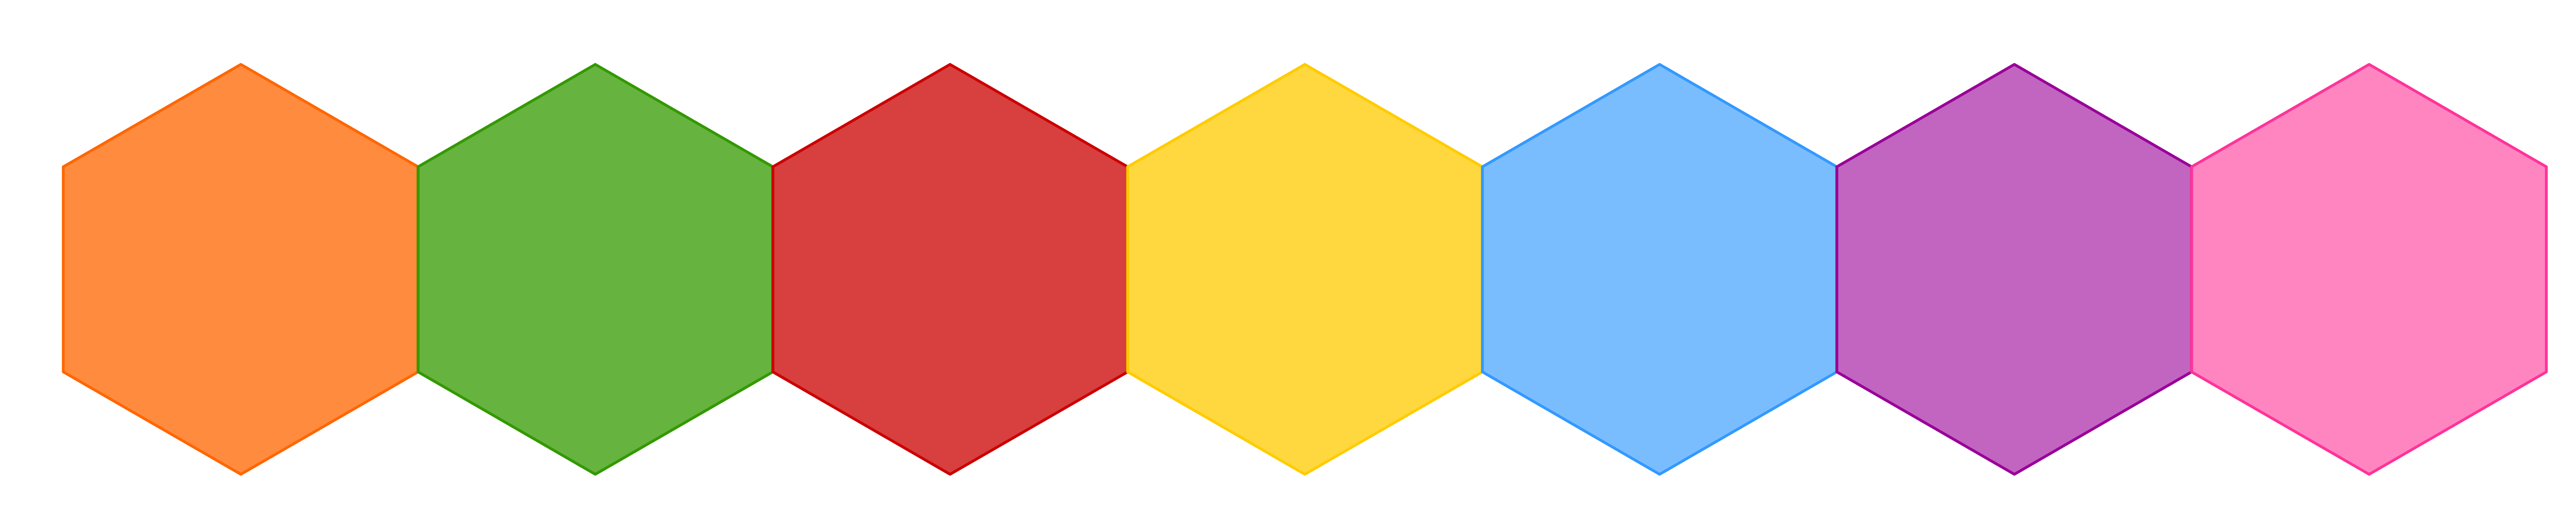
\includegraphics[scale = 0.12]{R2-1}
				\end{center}
				
				\noindent Диаметр каждого шестиугольника меньше~$1$, поэтому противоречий не~возникло.
				Распространим раскраску на~остальные шестиугольники: \\			
				\begin{center}
						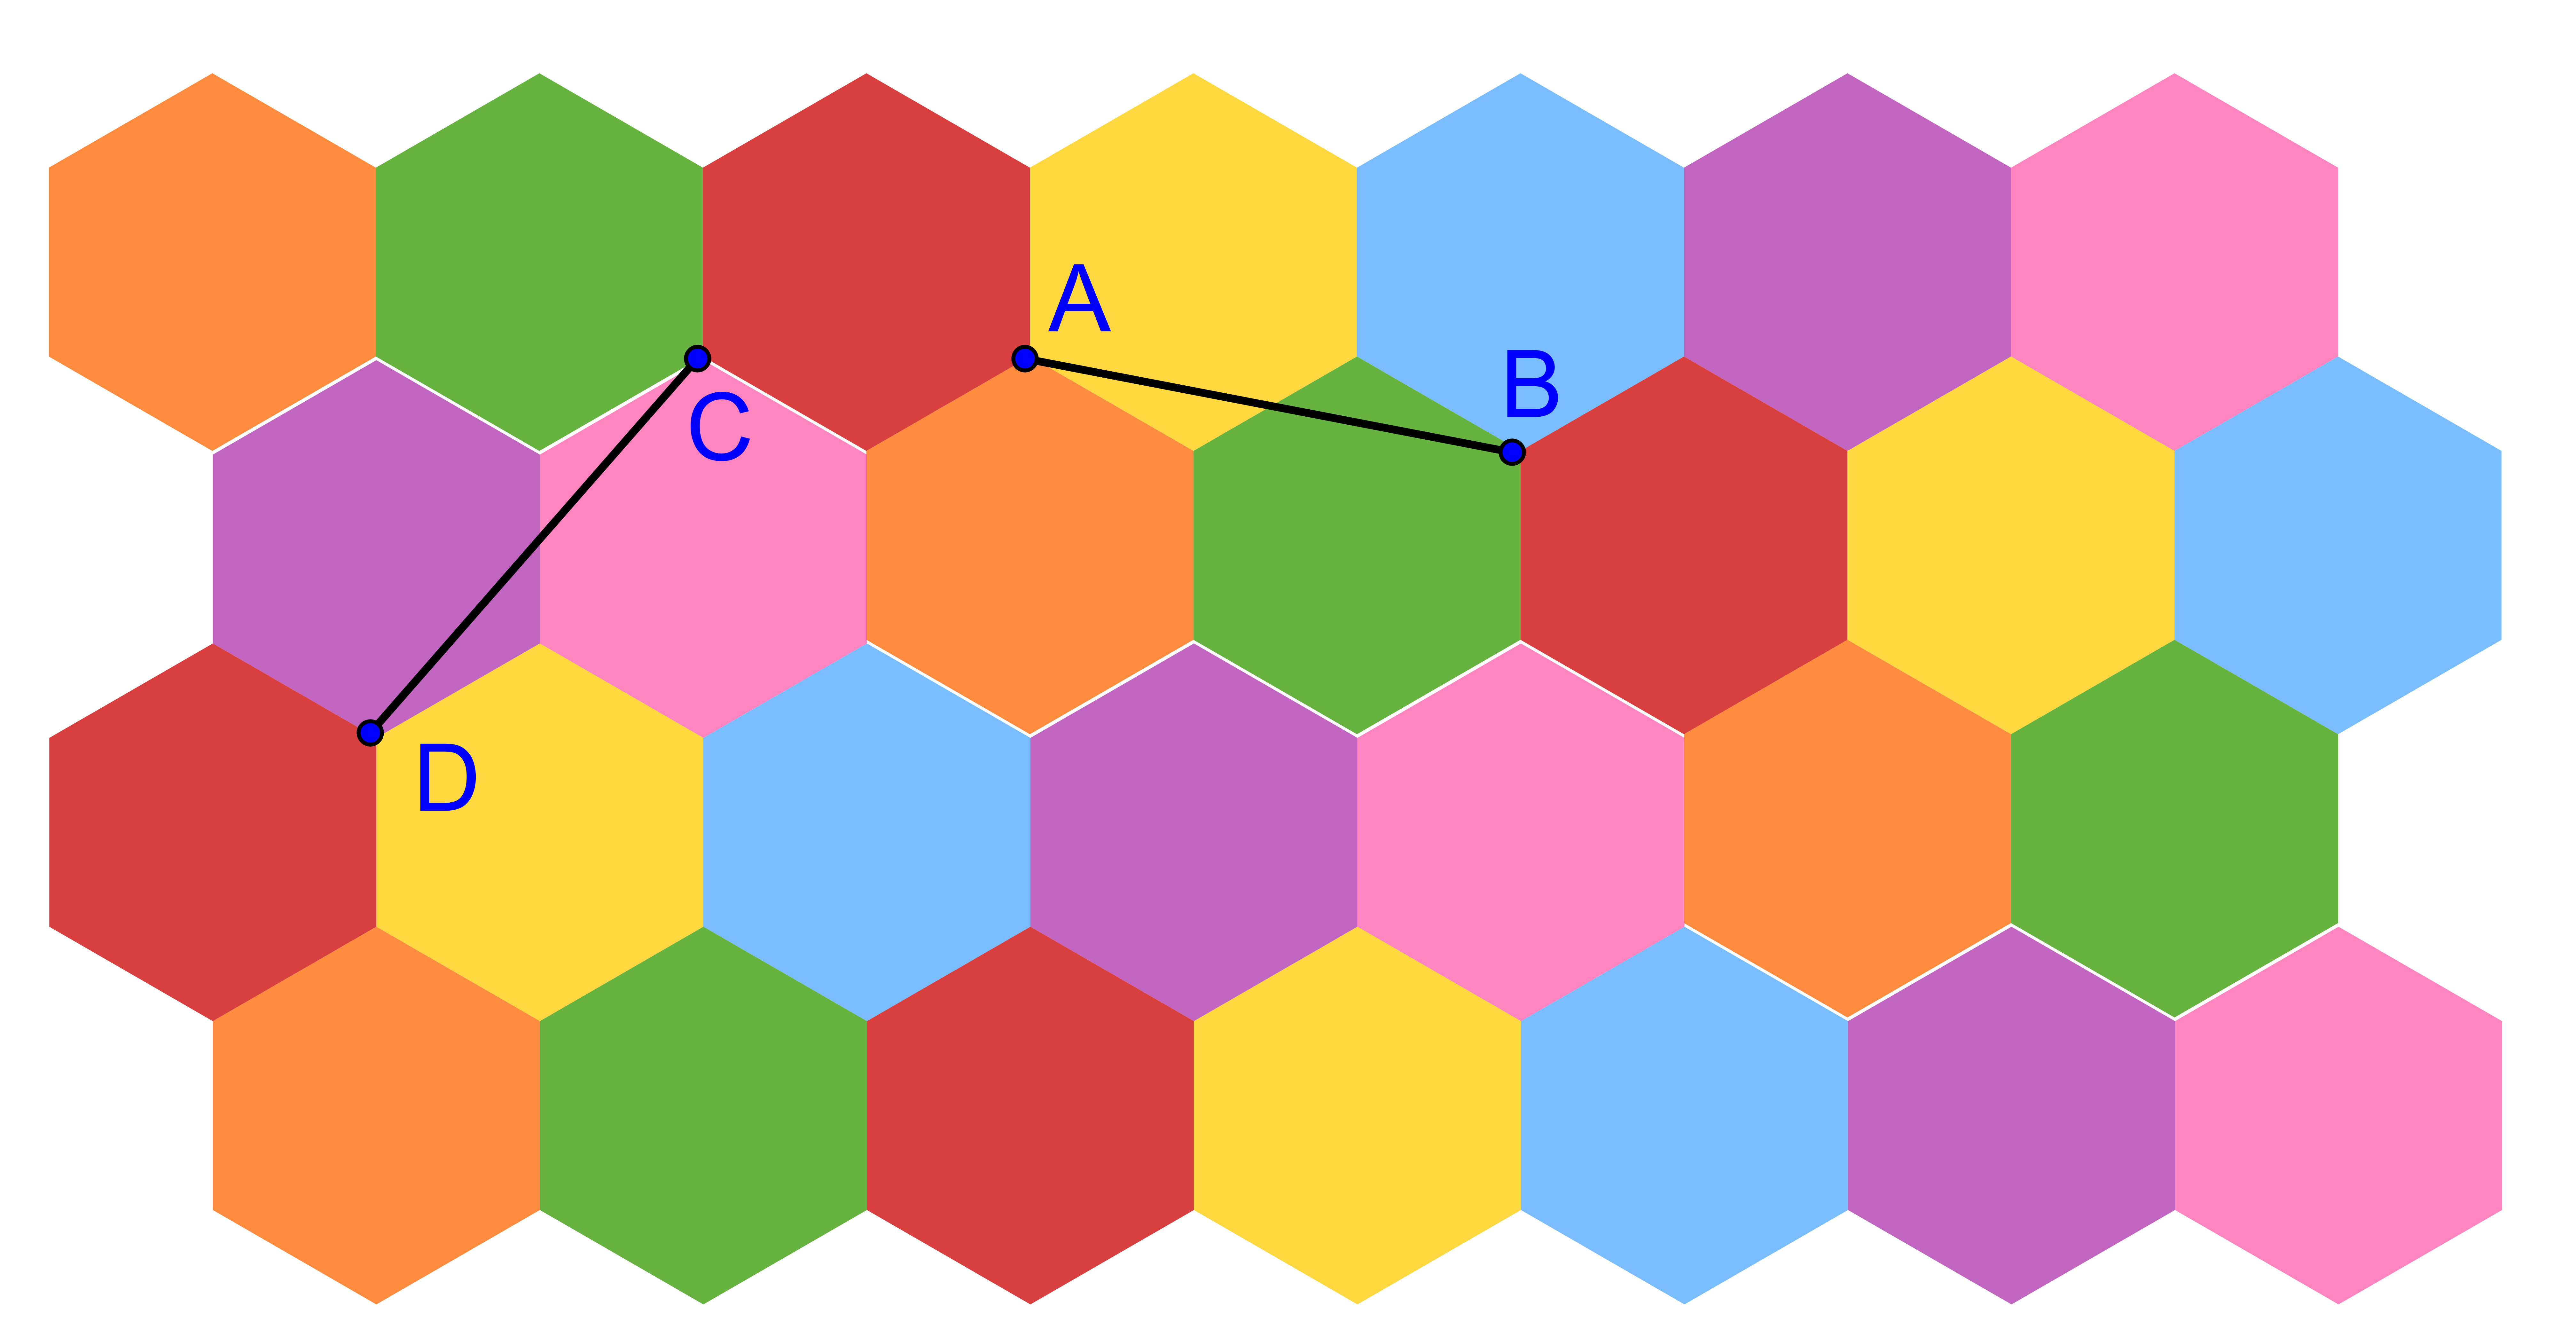
\includegraphics[scale = 0.12]{R2}
				\end{center}
				
				\noindent Нетрудно проверить, что расстояние между одноцветными точками разных 
				многоугольников больше единицы.
		\end{proof}
\end{claim}

\begin{claim}
		Для $n = 2$ выполнено $\chi(\mathbb{R}^2) \geq 4$ \\
		\begin{proof}
				Приведем дистанционный граф на~плоскости, так называемое 
				«Мозеровское веретено», для~раскраски которого трех цветов не~достаточно:\\
				\begin{center}
						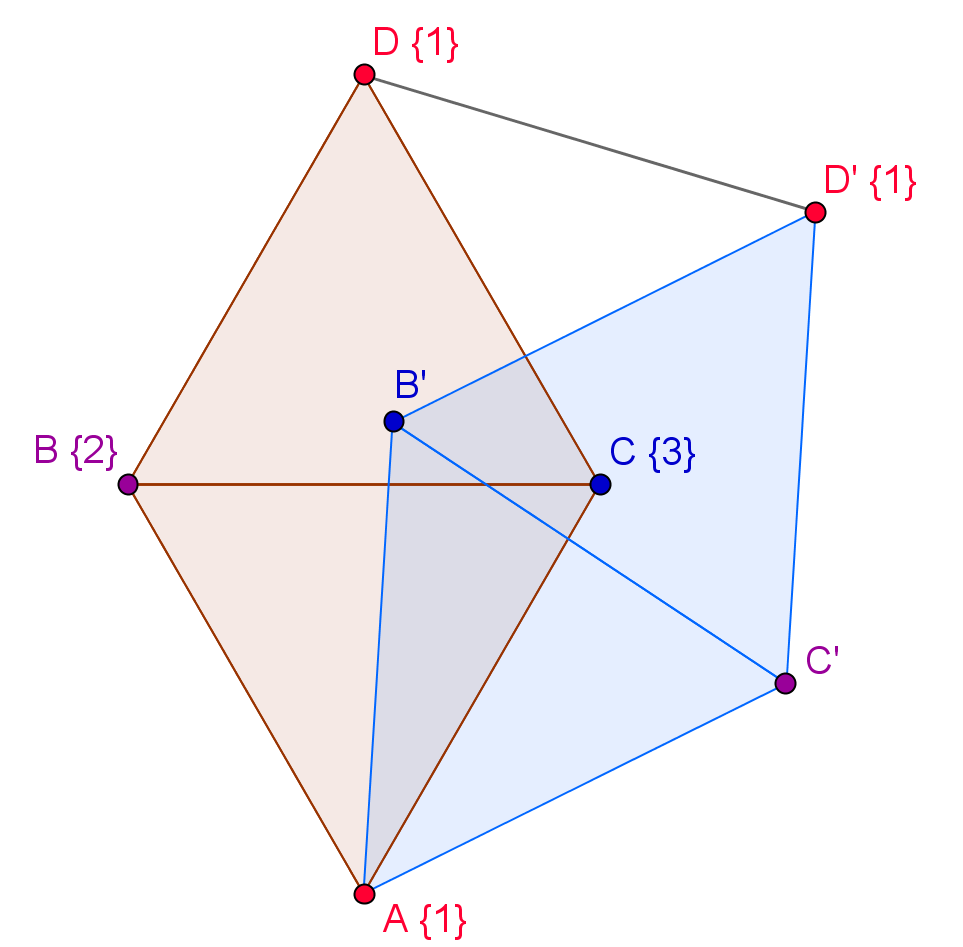
\includegraphics[scale = 0.6]{mozer}
				\end{center}
				
				\noindent Рассмотрим два треугольника $ABC$ и $DBC$ со~стороной~$1$, «склеенные» по~ребру. 
				Повернем конструкцию вокруг точки $A$ таким образом, чтобы точка $D$ и ее образ 
				находились на~расстоянии~$1$ друг от~друга.  Если точка~$A$ покрашена в~цвет~$\{1\}$,
				то точки $B$~и~$C$~– в~цвета $\{2\}$~и~$\{3\}$. Значит, точка~$D$~– первого цвета. Если 
				провести те~же рассуждения в~отношении точек $A, B', C', D'$, получим что и точка~$D'$
				первого цвета. Значит, раскраска не~правильная, т.к. $|DD'| = 1$ 
		\end{proof}
\end{claim}

\noindent Перейдем к оценкам для хроматического числа пространства $\mathbb{R}^3$.

\begin{claim}[Д.Е. Райский, 1970 г.]~\\
		Имеет место неравенство: $\chi(\mathbb{R}^3) \geq 5$ \\
		\begin{proof}
				Построим дистанционный граф, который будет являться трехмерным обобщением «мозеровского веретена». 
				Рассмотрим два правильных тетраэдра $ABCD$ и~$A'BCD$, «склеенные» по~грани.
				Пусть каждое ребро этих тетраэдров имеет длину~$1$. Повернем конструкцию вокруг точки~$A'$ так,
				чтобы точки~$A$ и~ее образ~$A''$ находились на~расстоянии~$1$ друг от~друга
				(образы точек при~повороте обозначены двумя штрихами). \\\\Предположим, что существует
				правильная раскраска полученного дистанционного графа в~4~цвета. Так~как вершины~$B, C, D$
				общей грани тетраэдров покрашены в~3 разных цвета, а~всего цветов~–~4,
				то точка~$A$ будет покрашена в~тот~же цвет, что и~точка~$A'$ (цвет~$\{1\}$).\\\\
				В~тетраэдре~$A'B''C''D''$ цвета точек~$B'', C'', D''$ отличны от~цвета точки~$A'$,
				значит, их цвета~–~$\{2\}$,~$\{3\}$~и~$\{4\}$ (не~обязательно соответственно).
				Следовательно, точка~$A''$ покрашена в~цвет~$\{1\}$, т.к. она удалена от~$B'',C'',D''$
				на~запрещенное для~одноцветных точек расстояние. \\
			\begin{center}
					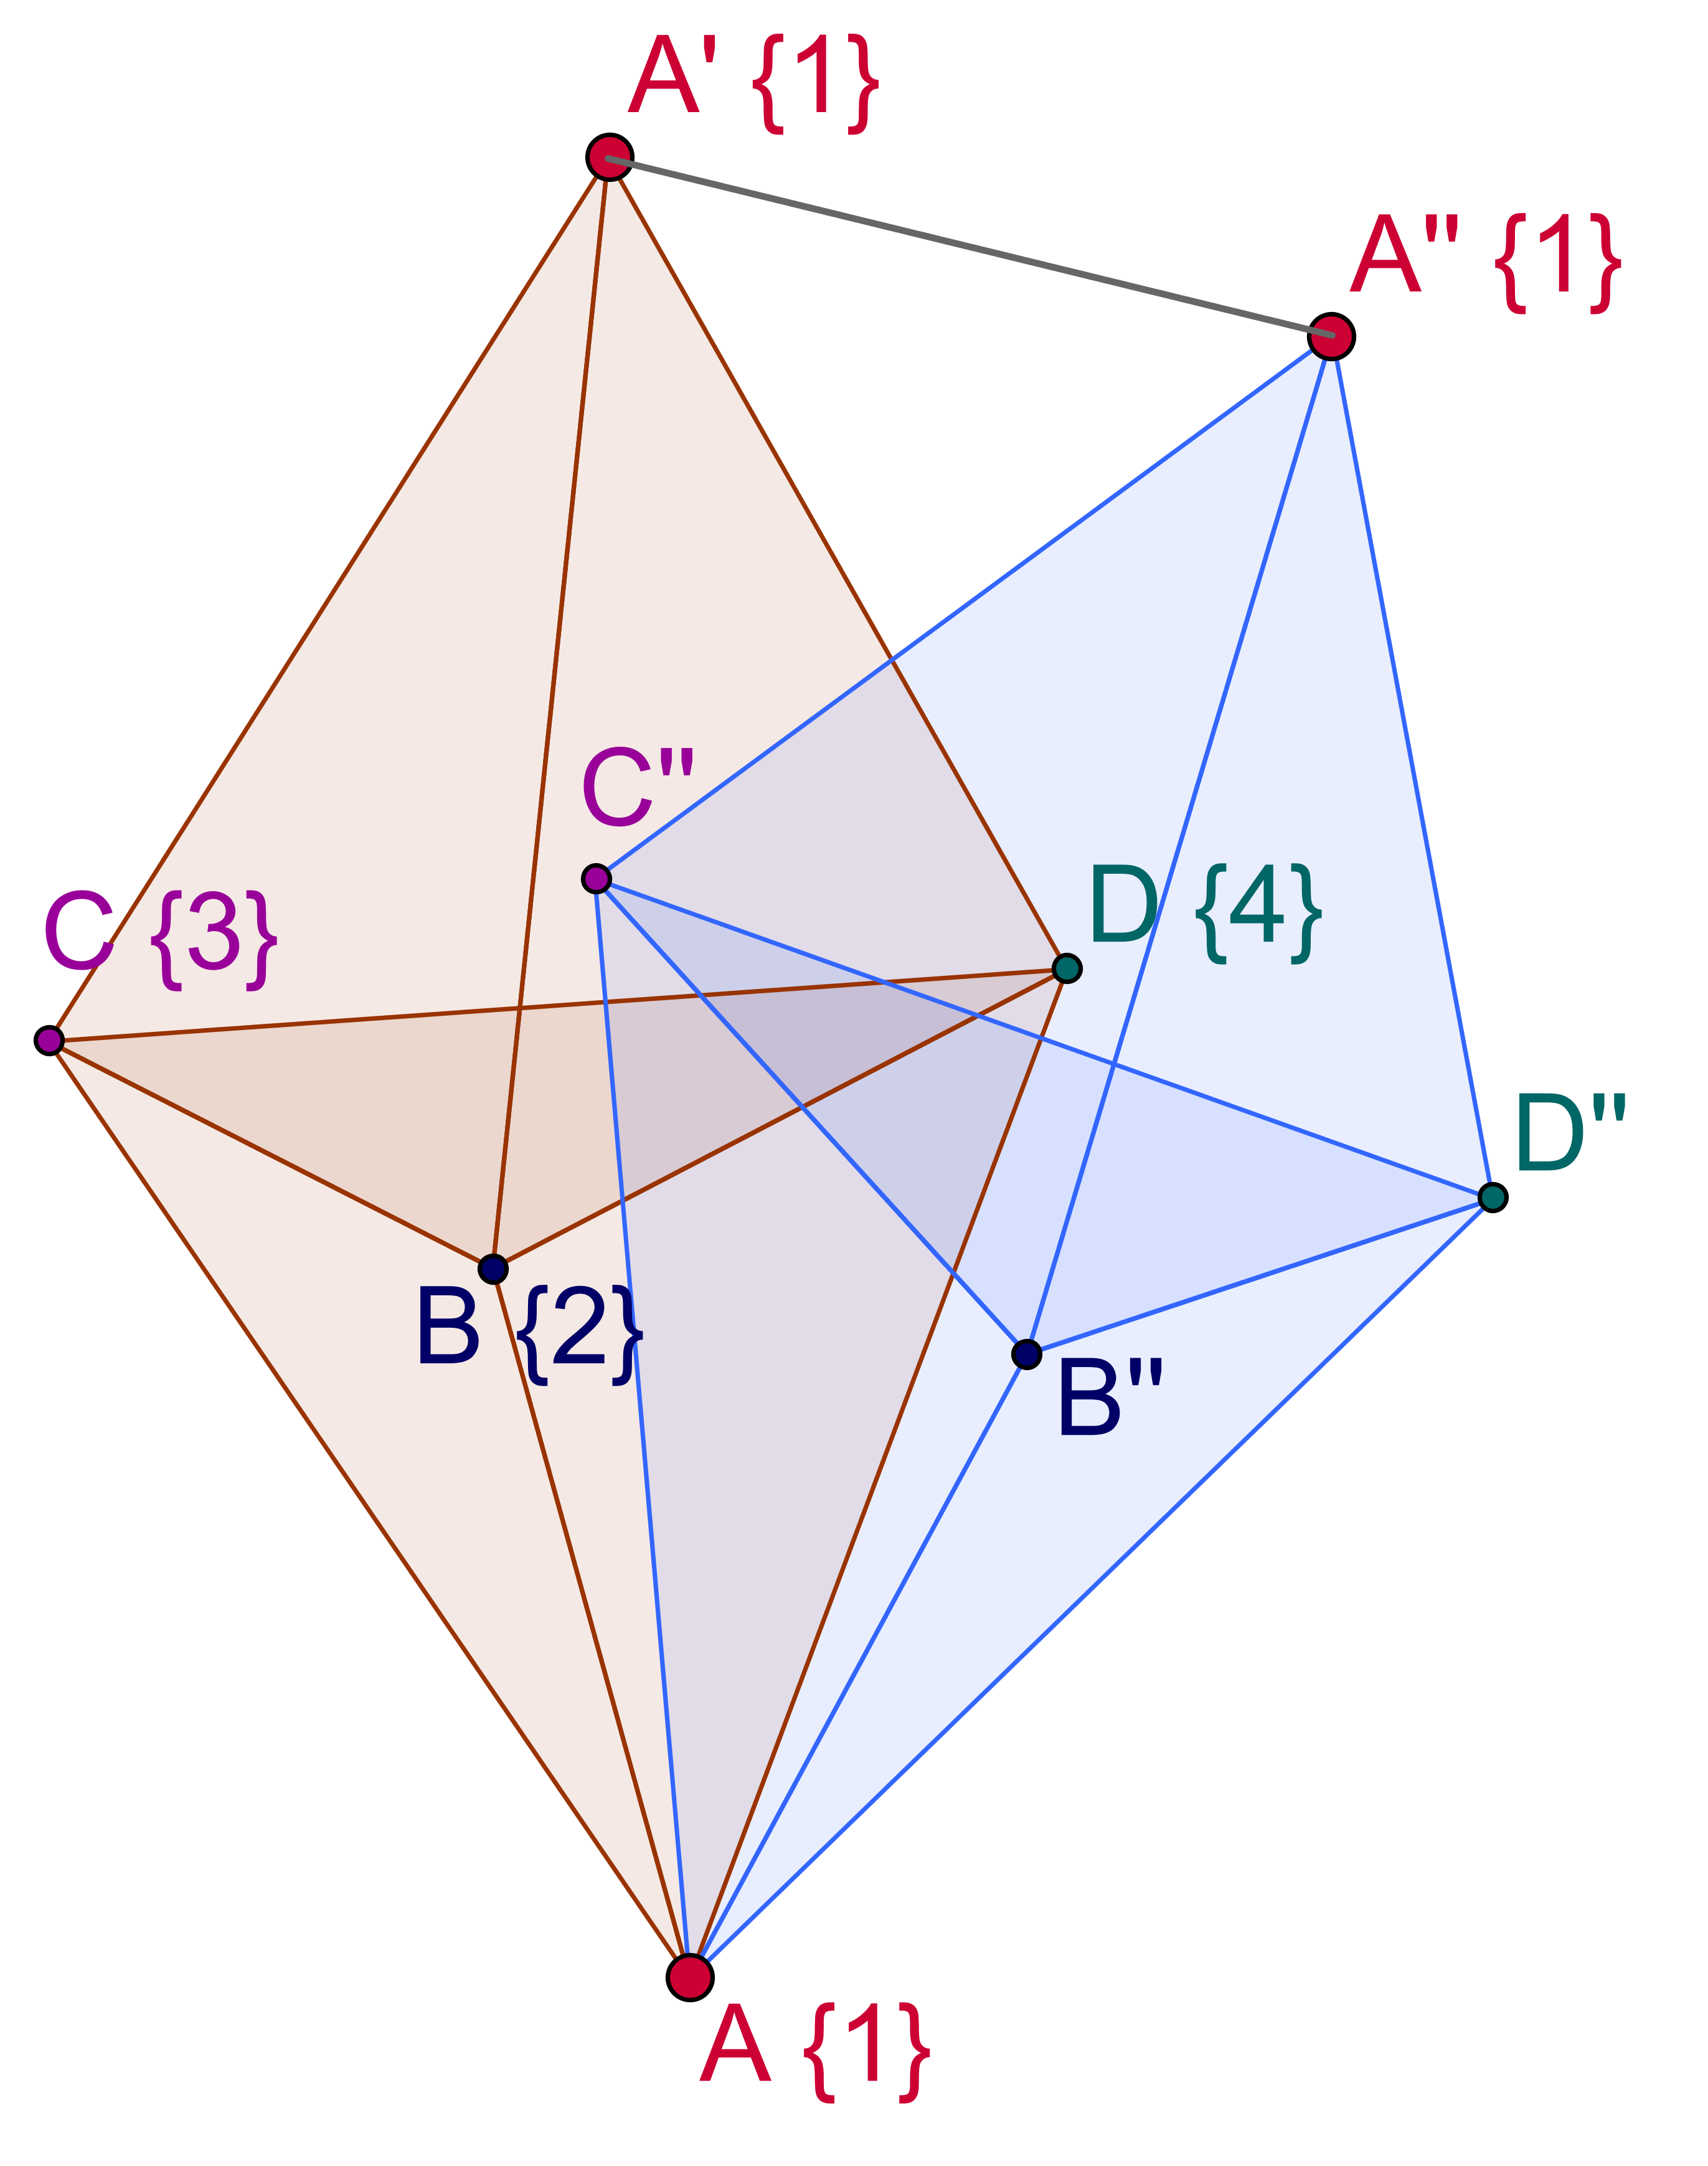
\includegraphics[scale = 0.23]{raisky}
			\end{center}
			
			\noindent Но~данная раскраска не~является правильной, т.к. можно указать две точки~$A$~и~$A''$
			на~единичном расстоянии, покрашенные в~один и~тот~же цвет. 	
		\end{proof}
\end{claim}

\begin{theorem}[О. Нечуштан, 2002 г, \cite{Nechushtan2002}]~\\
		Имеет место неравенство: $\chi(\mathbb{R}^3) \geq 6$ \\
		\begin{proof}
				Предположим, что существует правильная раскраска~$\mathcal{F}$ пространства в~5~цветов. 
				Рассмотрим пару точек~$S$~и~$T$ на~единичном расстоянии друг от~друга.
				Обозначим через~$\Omega$ множество точек, находящихся на~расстоянии~$1$ от $S$ и~от~$T$.
				Ясно, что~$\Omega$~– это окружность радиуса~$\frac{\sqrt{3}}{2}$, и на ней можно выбрать последовательность
				точек~$P, V, W, Q$ так, чтобы $|PV| = |VW| = |WQ| = 1$. Несложно вычислить,
				что $|PQ| = \frac{5}{3}$ и~$|PW| = |QV| = \sqrt{\frac{8}{3}}$. \\
				\begin{center}
						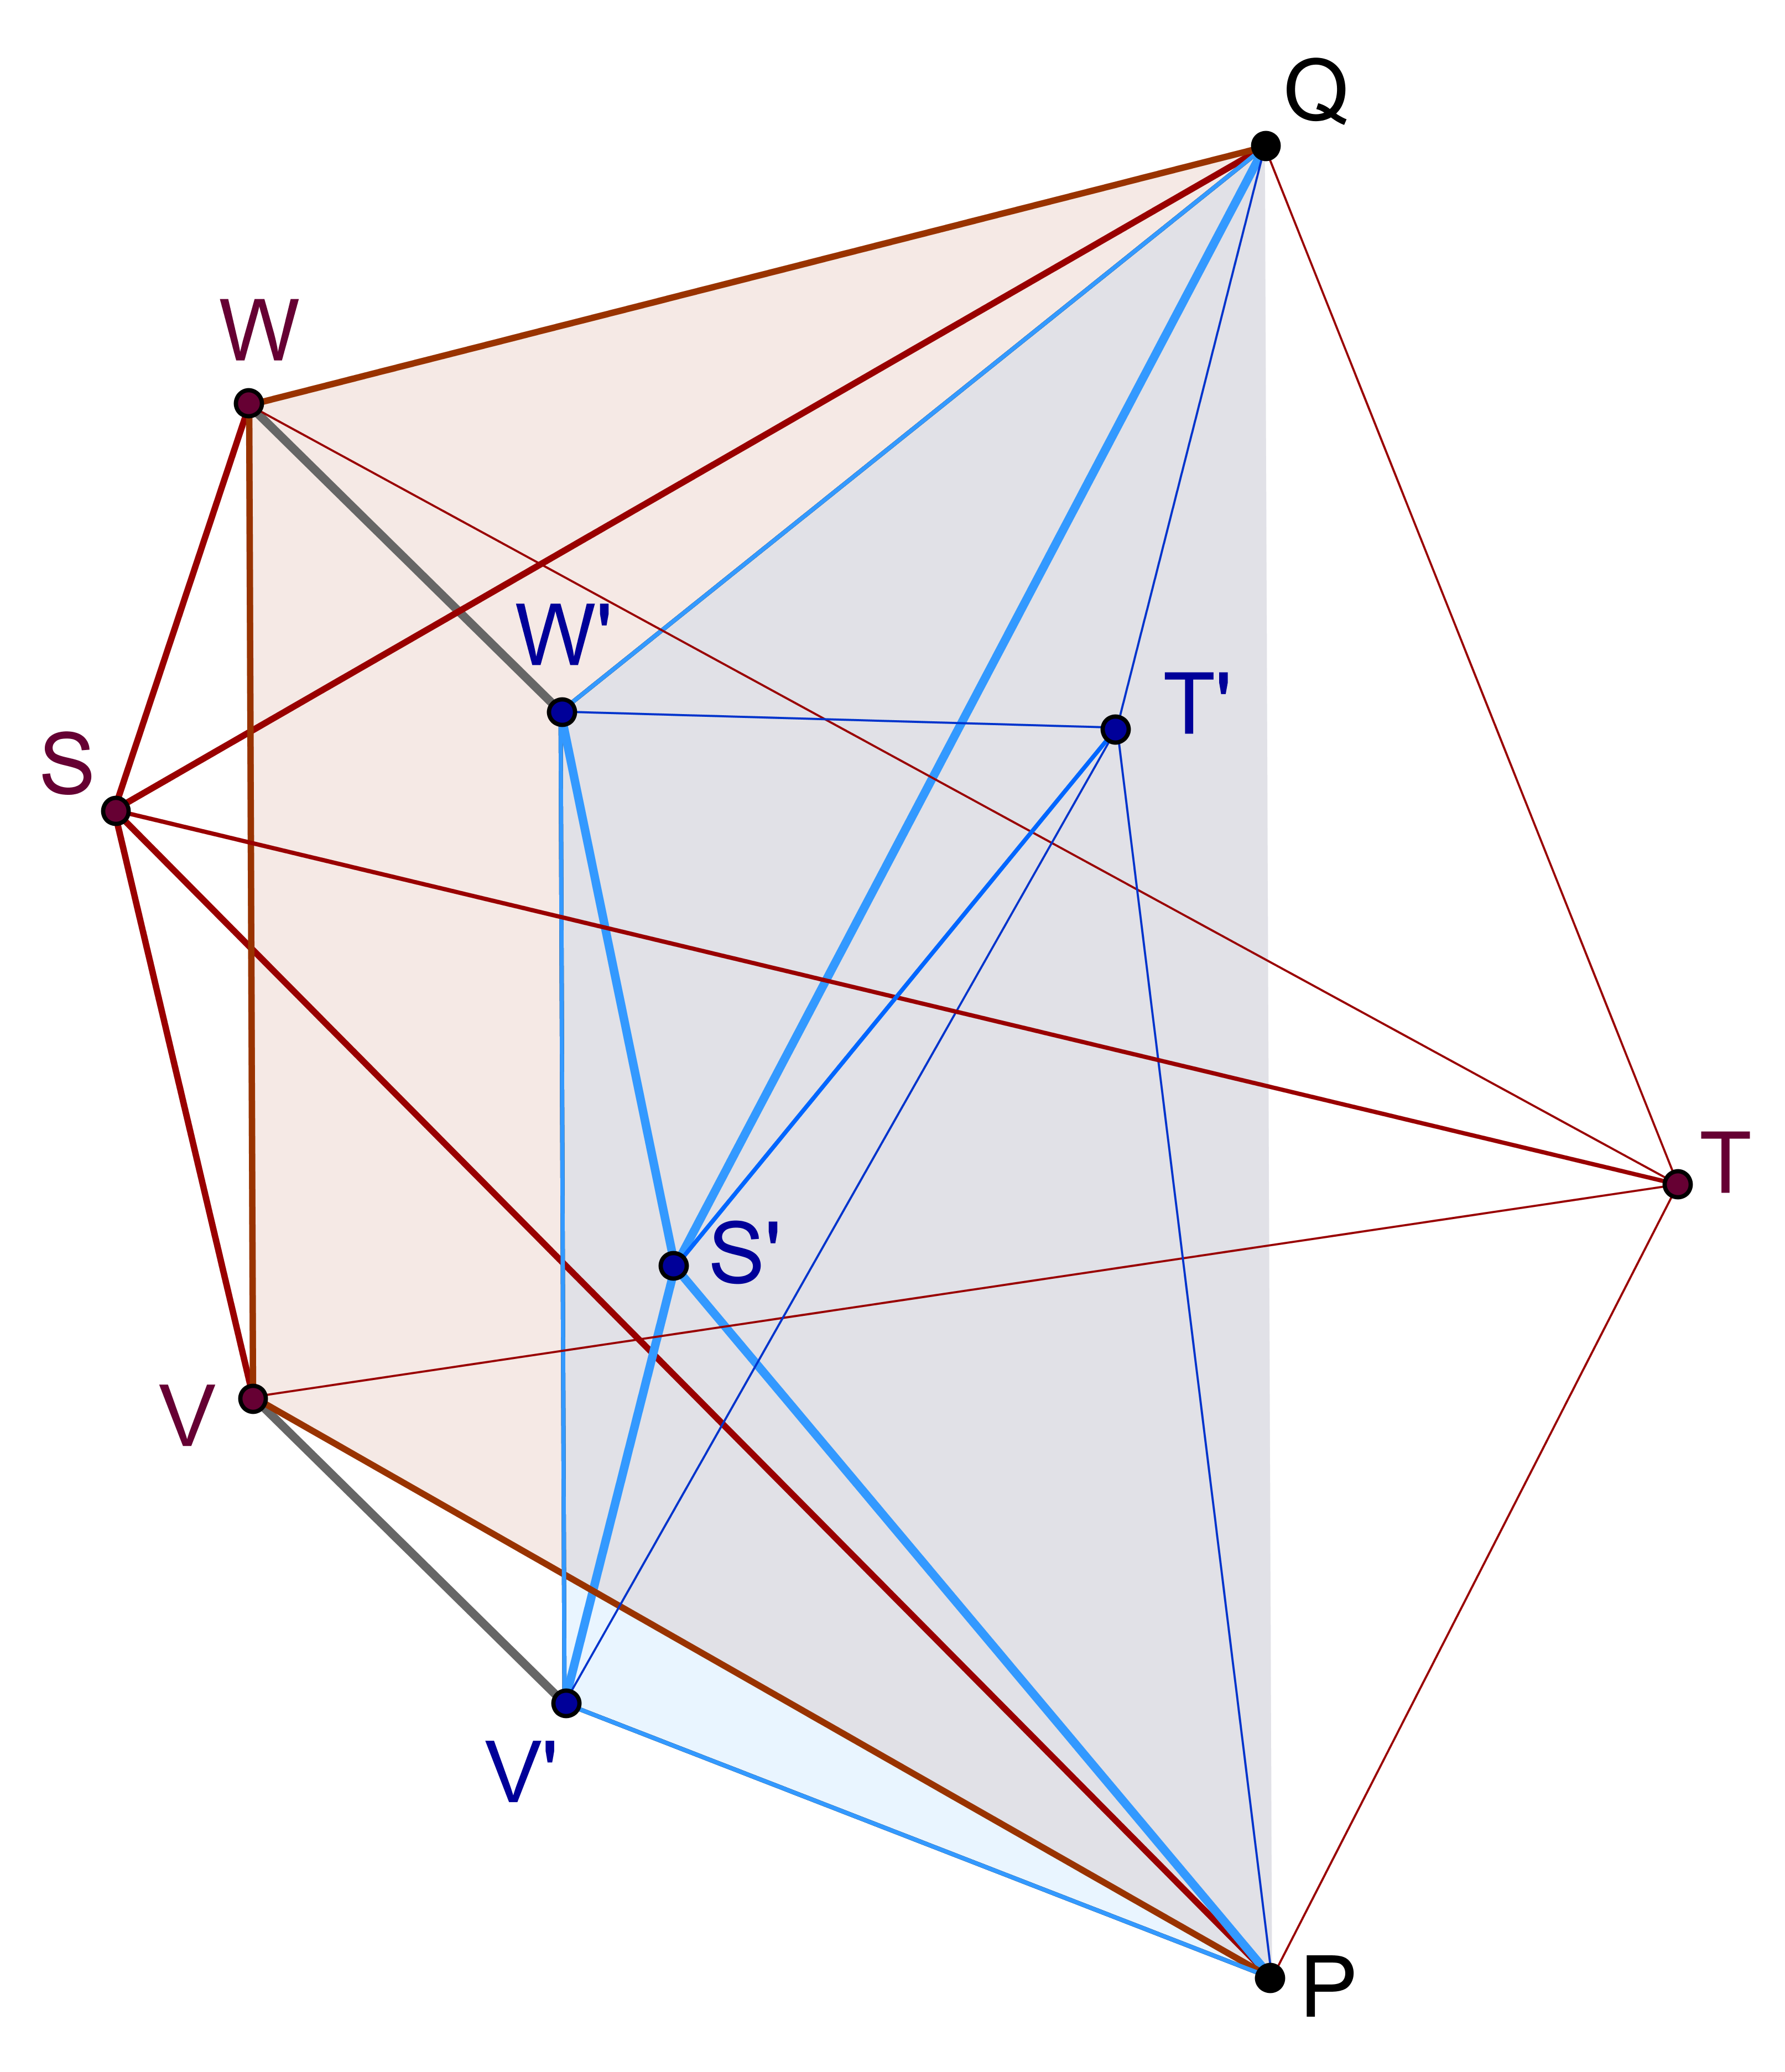
\includegraphics[scale = 0.25]{nechushtan}
				\end{center}
			
			  \noindent Повернем пространство вокруг прямой~$PQ$ так, чтобы точки~$V$ и ее образ~$V'$
				находились на~расстоянии~$1$ друг от~друга. Если образы точек при~повороте обозначить штрихами,
				то получим дистанционный граф $G = \{P, V, V', W, W' ,Q, S, S', T, T'\}$.\\\\
				\noindent Будем называть отрезок~$AB$ одноцветным, если его вершины покрашены в~один цвет,
				т.е. $\mathcal{F}(A) = \mathcal{F}(B)$, в противном случае~– разноцветным.
		\end{proof}
\end{theorem}
\newpage
\begin{lemma}
		Для любой правильной раскраски $\mathcal{F}$ в 5 цветов выполнено:
		\begin{enumerate}
				\item Если отрезок $PQ$ одноцветный, то отрезки $PW$, $QV$, $PW'$, $QV'$ разноцветные. 
				\item Среди отрезков $PQ$, $PW$, $QV$ ровно один одноцветный, как и среди отрезков $PQ$, $PW'$, $QV'$.
		\end{enumerate}
		\begin{proof}
				Первый пункт следует из~того, что отрезки~$PV$, $VW$, $WQ$ длины~$1$, и раскраска правильная.
				Точки~$S$~и~$T$ разного цвета, значит, для~раскраски~$\Omega$ запрещены 2~цвета.
				Следовательно, в~раскраске точек~$P$,~$Q$,~$V$,~$W$ используется не~больше трех цветов.
				Значит, найдется одноцветный отрезок с~вершинами в~этих точках. Это может быть только $PQ$, $PW$ или $QV$.
				Следовательно, среди $PQ$, $PW$, $QV$ (и, аналогично, среди $PQ$, $PW'$, $QV'$) есть хотя~бы один одноцветный.\\\\
				\noindent Если одноцветный отрезок~– это~$PQ$, то по~первому пункту леммы получаем, что он ровно один.
				Если $PQ$~– разноцветный, а $PW$ и $QV$ – одноцветны, то~отрезки $PW’$, $QV’$ (и еще $PQ$) – разноцветны.
				Но выше показано, что хотя~бы один одноцветный среди них есть. Получаем утверждение второго пункта леммы.
		\end{proof}
\end{lemma}

\noindent Обозначим через~$\Psi$ множество точек, удаленных от~$V$ и $V’$ на расстояние~1. Будем вращать окружность~$\Psi$ вокруг прямой~$PQ$, и полученное тело обозначим через~$\tau(\Psi)$.

\begin{lemma}
		Если $\mathcal{F}$ – правильная раскраска $\mathbb{R}^3$ в 5 цветов, и $\mathcal{F}(P) \ne \mathcal{F}(Q)$,
		то в раскраске $\tau(\Psi)$ не используется цвет точки $Q$. \\
		\begin{proof}
				Из леммы 1 следует, что один из отрезков $QV$ и $QV’$ будет одноцветным
				(иначе точки~$P$, $W$, $W’$ покрашены в~один и тот~же цвет).
				Так как на окружности~$\Psi$ нет цветов точек~$V$ и $V’$, то на~$\Psi$ нет цвета точки~$Q$.
				Эти~же рассуждения можно применить и для~образа окружности~$\Psi$ при~повороте.
				Получим, что в~раскраске~$\tau(\Psi)$ не~задействован цвет точки~$Q$.
		\end{proof}
\end{lemma}

\begin{proof}
		Рассмотрим в~пространстве две точки~$Q$ и $R$ на~расстоянии~$\frac{5}{3}$ друг от~друга.
		Обозначим через~$C$ следующую окружность: \\$C = \{X \in  \mathbb{R}^3 \mid |QX|= \frac{5}{3},|RX| = 1 \}$.
		Сначала рассмотрим случай, когда в~раскраске окружности~$C$ не используется цвет точки~$Q$. \\\\
		Для любой точки~$P$ на окружности~$C$ можно построить свое множество~$\tau(\Psi_P)$.
		Применив лемму~2, получим, что в~раскраске~$\tau(\Psi_P)$ не~используется цвет точки~$Q$.
		Объединяя множества~$\tau(\Psi_P)$ для каждой точки~$P$, лежащей на~окружности~$C$, получим некоторое множество~$T(\Psi)$: 
		\begin{equation}
				T(\Psi) = \{X \in \mathbb{R}^3 \mid \exists P \in C \colon X \in \tau(\Psi_P) \}.
		\end{equation}
		В~раскраске~$T(\Psi)$ не~используется цвет точки~$Q$. Можно показать, что множество~$T(\Psi)$ таково,
		что в~него можно поместить граф~Райского~– граф с~хроматическим числом, равным~5.
		Это значит, что на~покраску множества~$T(\Psi)$ вместе с~точкой~$Q$ потребуется как минимум~6 цветов.\\\\
		Если~же на~окружности~$C$ была точка~$R'$, покрашенная в~тот~же цвет, что и точка~$Q$,
		то ее и возьмем в~качестве точки~$R$ (точки окружности~$C$ были удалены от~$Q$ на то~же расстояние, что и точка~$R$).
		Тогда новая окружность~$C'$ (построенная по~$R’$) не~будет содержать точек, одноцветных с~$Q$, и задача
		сводится к~предыдущему случаю.
\end{proof}\\\\
\noindent Лучшая из~известных верхних оценок для~$\chi(\mathbb{R}^3)$ отличается от~нижней более чем вдвое:

\begin{theorem}[Д. Кулсон, 2000 г.]
		Выполнено соотношение $\chi(\mathbb{R}^3) \leq 15$
\end{theorem}

\noindent Дальше речь пойдет об~оценках хроматического числа в~больших размерностях, и нам понадобится понятие пестроты множества.

\begin{definition}
		Зафиксируем некоторое множество~$U \subset \mathbb{R}^n$. Пусть для правильной раскраски~$\mathcal{F}$
		число~$\pi_\mathcal{F}'(U)$~– это наибольшее такое~$k$, что найдется движение~$\mathcal{O}$ пространства~$\mathbb{R}^n$ такое,
		что число цветов, затраченное на~покраску множества~$\mathcal{O}(U)$ в~раскраске~$\mathcal{F}$, равно~$k$.
		Тогда пестротой множества~$U$ относительно пространства~$\mathbb{R}^n$ называют
		минимум чисел~$\pi_\mathcal{F}'(U)$ по~всем правильным раскраскам пространства~$\mathbb{R}^n$.
		\begin{equation}
				\pi^n(U) = \pi(U \mid \mathbb{R}^n) = \min_\mathcal{F}\max_\mathcal{O}\chi'(\mathcal{O}(U)),
		\end{equation} \\
		где~$\chi'(\mathcal{O}(U))$~– количество цветов, используемых в~раскраске~$\mathcal{F}$ при~покраске множества~$O(U)$.
\end{definition}

\begin{theorem}
		Имеет место неравенство: $\chi(\mathbb{R}^4) \geq 7$ \\
		Покажем, как можно доказать эту теорему, если известна оценка на пестроту сферы.
\end{theorem}

\begin{lemma}[А.Б. Купавский, \cite{Kupavsky2011}]
		При $n \geq 4$ и $r > \frac{1}{2\sqrt{\sqrt{3}-1}}, r \ne \sqrt{\frac{3}{8}}$ , верна оценка
		\begin{equation}
				\pi^n(S_r^2) \geq 5.
		\end{equation}
		
		\begin{proof}
				Из леммы~3 следует, что при~любой правильной раскраске~$\mathbb{R}^4$
				найдется двумерная сфера~$S^2$ радиуса~$\frac{\sqrt{3}}{2}$, при раскраске которой используется 5~цветов.
				Через центр этой сферы можно провести прямую, ортогональную трехмерной гиперплоскости, содержащей сферу.
				На~этой прямой можно отметить две точки~$A$ и~$B$ на~расстоянии~$\frac{1}{2}$ от~центра сферы, а,
				значит, на~единичном расстоянии друг от~друга: \\
				\begin{center}
						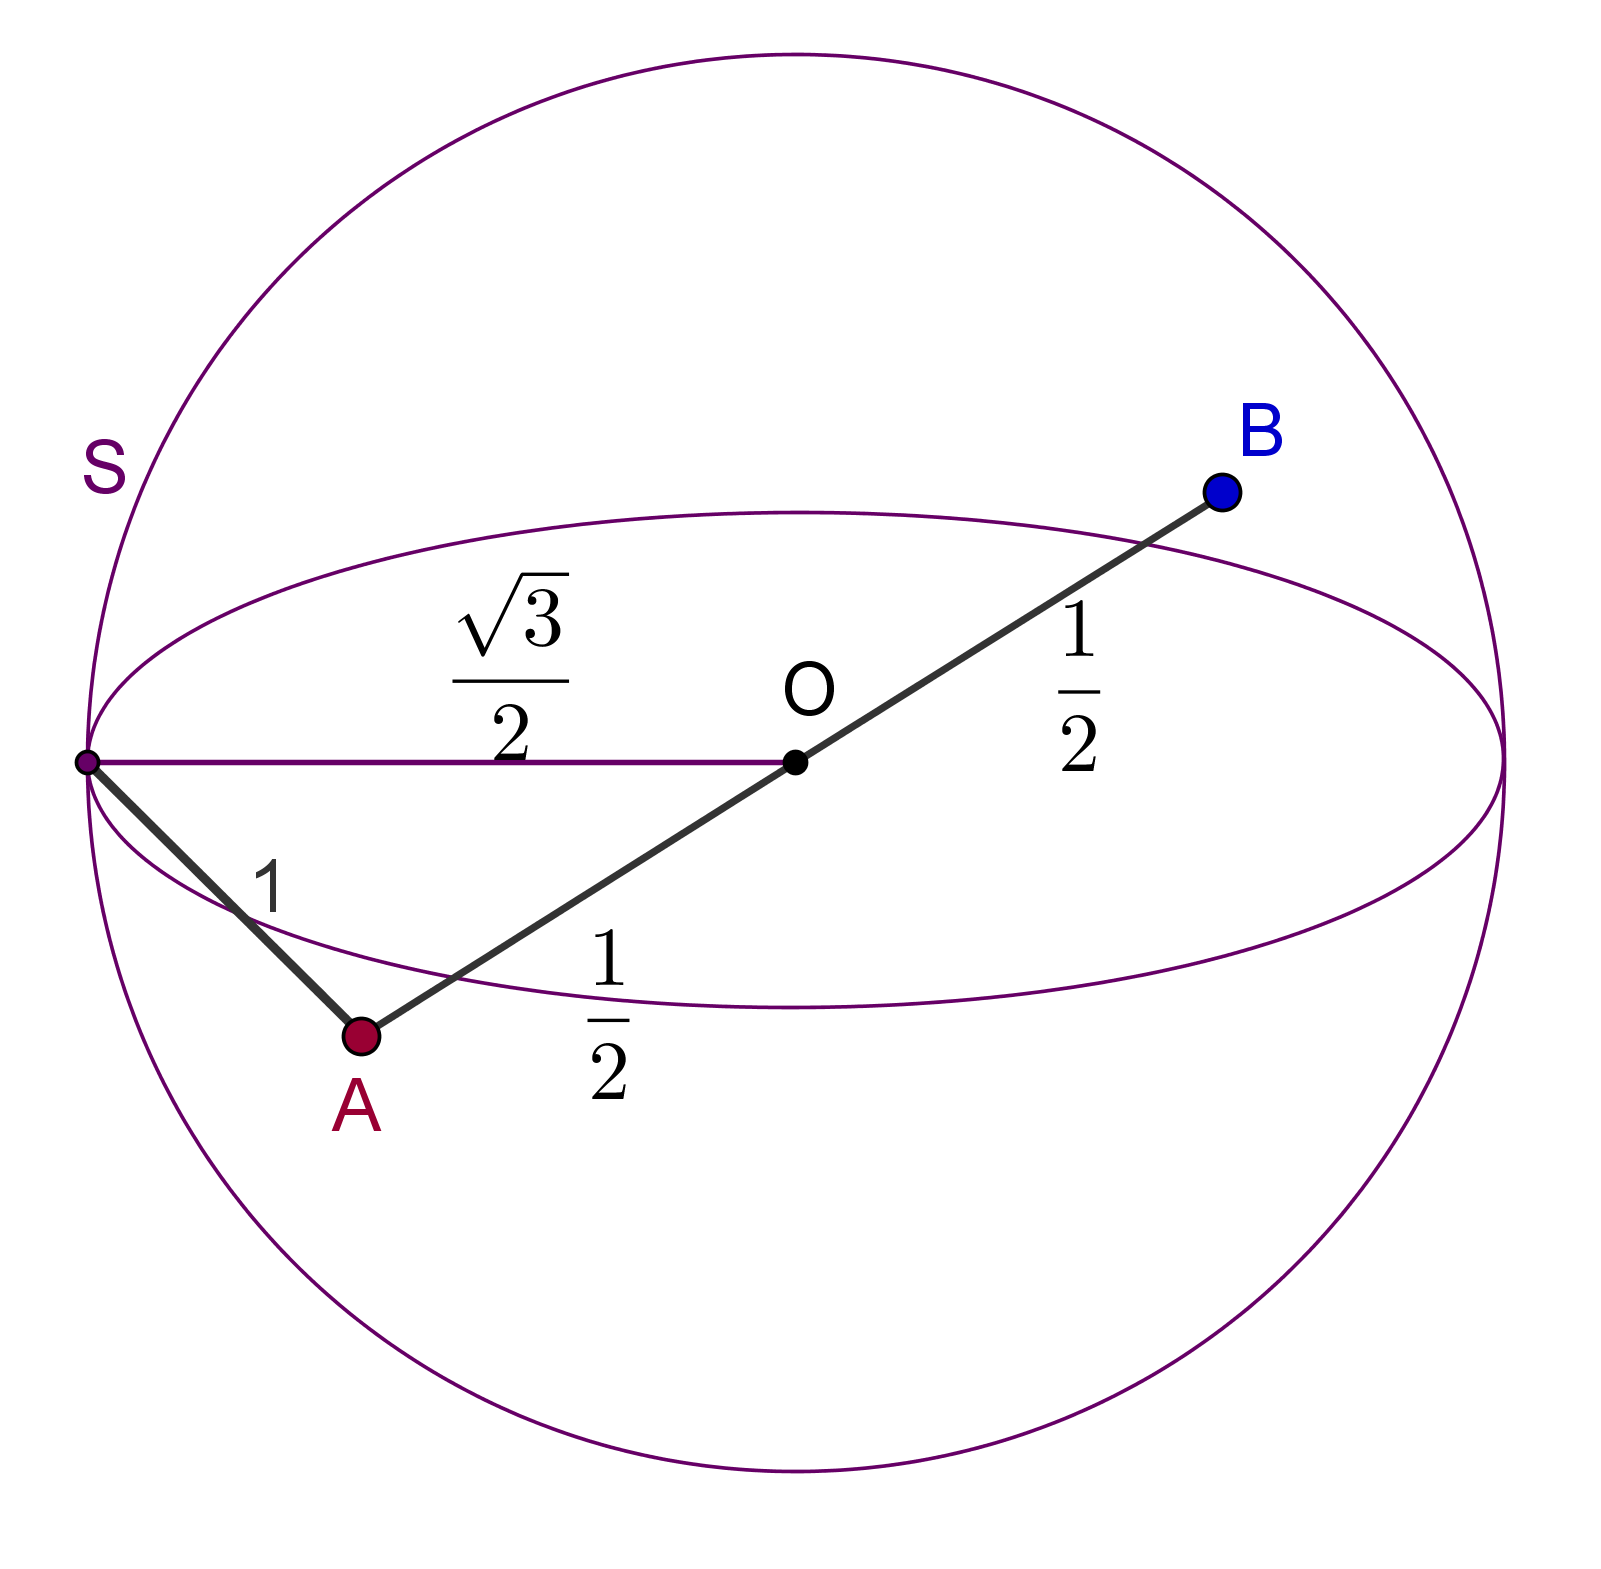
\includegraphics[scale = 0.25]{R4}
				\end{center}
				
				\noindent При~заданном радиусе точки сферы~$S^2$ будут находиться на~расстоянии~$1$ от точек $A$ и $B$.
				Значит, необходимо как минимум 7 различных цветов ($\chi(S^2) \geq 5$ и ещё 2 цвета – для покраски точек $A$, $B$). 
		\end{proof}
\end{lemma}

\noindent Теперь покажем, как можно получить оценки на~пестроту самих сфер (в~зависимости от~радиуса и размерности пространства, в~которое сфера вложена). Не~будем приводить вычислений для~допустимого радиуса~r сферы, отметим лишь, что радиус~r и размерность пространства подобраны таким образом, чтобы описанные ниже конструкции было возможно реализовать. Будем ссылаться на~следующую лемму:

\begin{lemma}[А.Б. Купаский, \cite{Kupavsky2011}]
		Пусть $Sp_x^n$ – правильный $n$-мерный симплекс со стороной $x$,
		а радиус описанной вокруг него сферы равен $\alpha$. Тогда для любого $\alpha > \frac{n}{2n + 2}$
		\begin{equation}
				\pi^{2n}(Sp_x^n) = n+1
		\end{equation}
\end{lemma}

\begin{theorem}[А.Б. Купавский \cite{Kupavsky2011}]~\\
		При $n > 7$ и
		$r \in \left(\sqrt{\frac{\left(1+\sqrt{\frac{\vphantom{2} n}{2(n+1)}}\right)^2}{n^2+6n+4+\sqrt{8n(n+1)}}+\frac{n}{2n+2}},
													\sqrt{\vphantom{\frac{\left(1+\sqrt{\frac{n}{2(n+1)}}\right)^2}{n^2+6n+4+\sqrt{8n(n+1)}}} \frac{\left(\sqrt{\vphantom{2} n+2} + \sqrt{\vphantom{n+} 2}\right)^2+n^3}{(2n+2)n^2}}\right)$ выполнено:
		\begin{equation}
				\pi^{2n+2}(S_r^n) \geq 2n+2
		\end{equation}
		\begin{proof}
				Зафиксируем правильную раскраску~$\mathbb{R}^{2n+2}$, радиус~$r$ из~теоремы и будем искать сферу~$S_r^n$,
				покрашенную в~$2n+2$ цвета. Из леммы~4 следует,
				что при некоторых условиях на~радиус~$\alpha$ описанной сферы найдется $n$-мерный симплекс~$Sp^n$ (далее обозначен как~$W$),
				покрашенный в~$n+1$ цвет. Описанную вокруг этого симплекса сферу обозначим~$S^{n-1}$.
				Сфера~$S^{n-1}$ содержится в~некоторой сфере~$S_r^n$.
				При фиксированном радиусе~$r$ можно подобрать радиус~$\alpha$ сферы~$S^{n-1}$ таким образом,
				чтобы в~$S_r^n$ содержалось множество~$V$ из~$n + 1$ точки со~свойствами:
				\begin{enumerate}
						\item Точки множества~$V$ удалены друг от~друга на~расстояние~$1$, то~есть, образуют единичный симплекс~$Sp_1^n$.
						\item Каждая точка множества~$V$ удалена от~$n$ вершин симплекса~$W$ на расстояние~$1$,
									то~есть, удалена на~расстояние, отличное от~единицы, только от~одной вершины симплекса~$W$.
				\end{enumerate}
				Итак, множество~$V$~– это симплекс~$Sp_1^n$ со~стороной~$1$.
				Описанная вокруг него сфера~$S_{r'}^{n-1}$ (вложенная в~$S_r^n$) лежит в~$n$-мерной плоскости,
				параллельной аналогичной плоскости для~$S^{n-1}$.\\\\
				\noindent Будем вращать симплекс~$V$ вокруг плоскости, содержащей $S^{n-1}$.
				Каждая вершина~$v$ симплекса~$V$ опишет~$(n+1)$-мерную сферу,
				в~которую можно вписать $(n+1)$-мерный симплекс~$Sp_1^{n+1}$ со стороной~$1$.
				Поэтому можно выбрать только те повороты $o_1$, $o_2$, $\ldots$, $o_{n+2}$ пространства,
				которые переводят вершину~$v$ в~вершины симплекса~$Sp_1^{n+1}$.
				Множество таких вращений обозначим~$\mathcal{O}$, а~симплекс, полученный в~результате применения
				вращений из~$\mathcal{O}$ к~вершине~$v$, обозначим~$\mathcal{O}(v)$. \\
				\begin{center}
						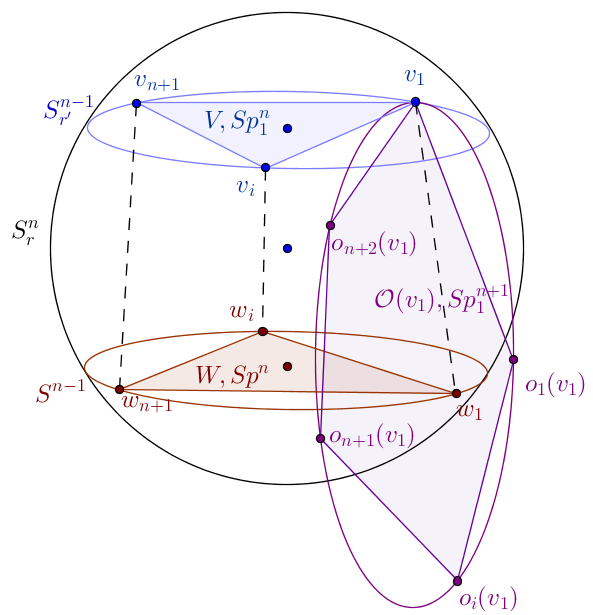
\includegraphics[scale = 1]{sphere}
				\end{center}
				
				\noindent Для~каждой вершины~$v_i$ симплекса~$V$ $( i \in \{1, 2, \ldots, n+1\})$ обозначим через~$w_i$ ту единственную вершину симплекса~$W$,
				расстояние до~которой отлично от~$1$. Так как цвета точек $o_1(v_i)$, $o_2(v_i)$, $\ldots$, $o_{n+2}(v_i)$ различны,
				то среди этих точек можно выбрать как минимум $n+1$ точку, покрашенную не в~цвет~$w_i$.
				Получаем для~каждой вершины~$v_i$ симплекса~$V$ $(n+1)$-элементное подмножество точек $(n+2)$-элементного множества~$\mathcal{O}(v_i)$.
				Симплекс~$V$ имеет $n+1$ вершину, значит, по~принципу~Дирихле, найдется поворот, например,~$o_1$,
				при котором $o_1(v_i)$ и~$w_i$ покрашены в~разные цвета для~любого~$i$.
				Симплексы~$o_1(V)$ и~$W$ вложены в~некоторую $n$-мерную сферу~$S_r^n$, на покраску которой затрачено $2n+2$~цвета,
				т.к. любые две вершины симплексов~$o_1(V)$ и~$W$ покрашены в~разные цвета. 
		\end{proof}
\end{theorem}

\noindent Покажем, что можно обобщить доказательство теоремы~4 на~случай, 
когда семейство~$\mathcal{O}$ вращений переводит вершину~$v$ в~некоторый дистанционный граф~$G(v)$ 
с~хроматическим числом, не~меньшим~$n + 2$. В~частности, в~качестве~$G(v)$ 
можно рассмотреть единичный симплекс~$Sp_1^{n+1}$, что и было сделано при~доказательстве теоремы~4.

\begin{claim}
		Пусть симплексы $W$ и $V$ располагаются в~пространстве так, как было описано в~доказательстве теоремы~4.
		Рассмотрим семейство~$\mathcal{O}$ вращений вокруг плоскости, содержащей симплекс~$W$, таких,
		что образы каждой вершины~$v_i$ образуют дистанционный граф~$G(v_i)$, причём $\chi(G(v_i)) \geq n+2$.
		Тогда существует такое вращение~$o \in \mathcal{O}$, что для~любого~$i \in \{1, 2, \ldots, n + 1\}$ цвет~$w_i$ не~совпадает с~цветом~$o(v_i)$. \\
		\begin{proof}
				Сначала выберем из~семейства~$\mathcal{O}$ те и только те вращения, при~которых образ вершины~$v_1$ покрашен в~цвет,
				отличный от~цвета~$w_1$. Полученное множество вращений обозначим~$\mathcal{O}_1$.
				Заметим, что для~каждой вершины~$v_i$ симплекса~$V$ граф~$\mathcal{O}_1(v_i)$ имеет хроматическое число, равное, по~крайней мере,~$n+1$.
				Действительно, если это не~так, и~существует правильная раскраска~$\mathcal{O}_1(v_i)$ в~$n$ цветов,
				то раскрасим в~новый $(n+1)$-й цвет (пусть – черный) образы вершины~$v_i$ при вращениях из множества $\mathcal{O}\!\setminus\!\mathcal{O}_1$.
				Полученная раскраска графа~$G(v_i)$ в~$n+1$ цвет будет правильной,
				т.к. любые две~вершины черного цвета удалены друг от~друга на~незапрещенное расстояние.
				Это так, потому что при~правильной раскраске графа~$\mathcal{O}(v_1)$ аналогичные им вершины (получающиеся при тех~же вращениях пространства)
				были покрашены в~один и тот~же цвет. Итак,~$\chi(\mathcal{O}_1(v_i)) \geq n+1$. \\\\
				\noindent Далее построим аналогично множество~$\mathcal{O}_2$ для вершины~$v_2$: из множества~$\mathcal{O}_1$ выберем те и только те вращения,
				при~которых цвет образа вершины~$v_2$ отличен от~цвета~$w_2$. Можно провести аналогичные рассуждения и получить,
				что хроматическое число графа~$\mathcal{O}_2(v_i)$ не меньше~$n$ (для~всех вершин~$v_i$).
				Продолжим строить по~аналогии множества $\mathcal{O}_3$, $\mathcal{O}_4$, $\ldots$, $\mathcal{O}_{n+1}$.
				При~переходе к~каждому следующему множеству хроматическое число графа $\mathcal{O}_{j+1}(v_i)$
				будет не~более чем на $1$ меньше хроматического числа графа~$\mathcal{O}_j(v_i)$.
				Таким образом, $\chi(\mathcal{O}_{n+1}(v_i)) \geq ((n+2)-(n+1)) = 1$. Это означает, что множество~$\mathcal{O}_{n+1}$ не~пусто,
				и существует поворот $o \in \mathcal{O}_{n+1} \subset \ldots \subset \mathcal{O}_2 \subset \mathcal{O}_1 \subset \mathcal{O}$,
				при~котором цвета~$o(v_i)$ и~$w_i$ отличаются. 
		\end{proof}
\end{claim}
\newpage
\section{Новые результаты}

Результаты данного раздела, возможно, являются фольклорными, однако автор не~встречал их в~литературе по~данной тематике.

\begin{claim}
		При любой правильной раскраске плоскости найдется прямая~$l$, в раскраске которой используется хотя~бы~3 различных цвета:
		\begin{equation}
				\pi^2(l) \geq 3
		\end{equation}
		\begin{proof}
				Предположим, что существует правильная раскраска плоскости такая,
				что любая прямая раскрашена ровно в~2 цвета (прямая не~может быть покрашена в~один цвет,
				т.к. на~ней есть точки на~расстоянии~$1$). Рассмотрим правильный треугольник~$ABC$ со~стороной длины~$1$.
				Прямые, содержащие его~стороны, разбивают  плоскость на~7 частей.
				Так как плоскость нельзя покрасить в~число цветов, меньшее~4, то можно выбрать точку~$D$,
				цвет которой будет отличаться от~тех трех цветов, использующихся для раскраски~$ABC$.
				Если точка~$D$ лежит на~одной из~проведенных прямых, то эта прямая и будет раскрашена как минимум в~3 цвета.
				Без ограничения общности, остается рассмотреть три случая расположения точки~$D$ (все три случая изображены на~одном рисунке): \\
				\begin{center}
						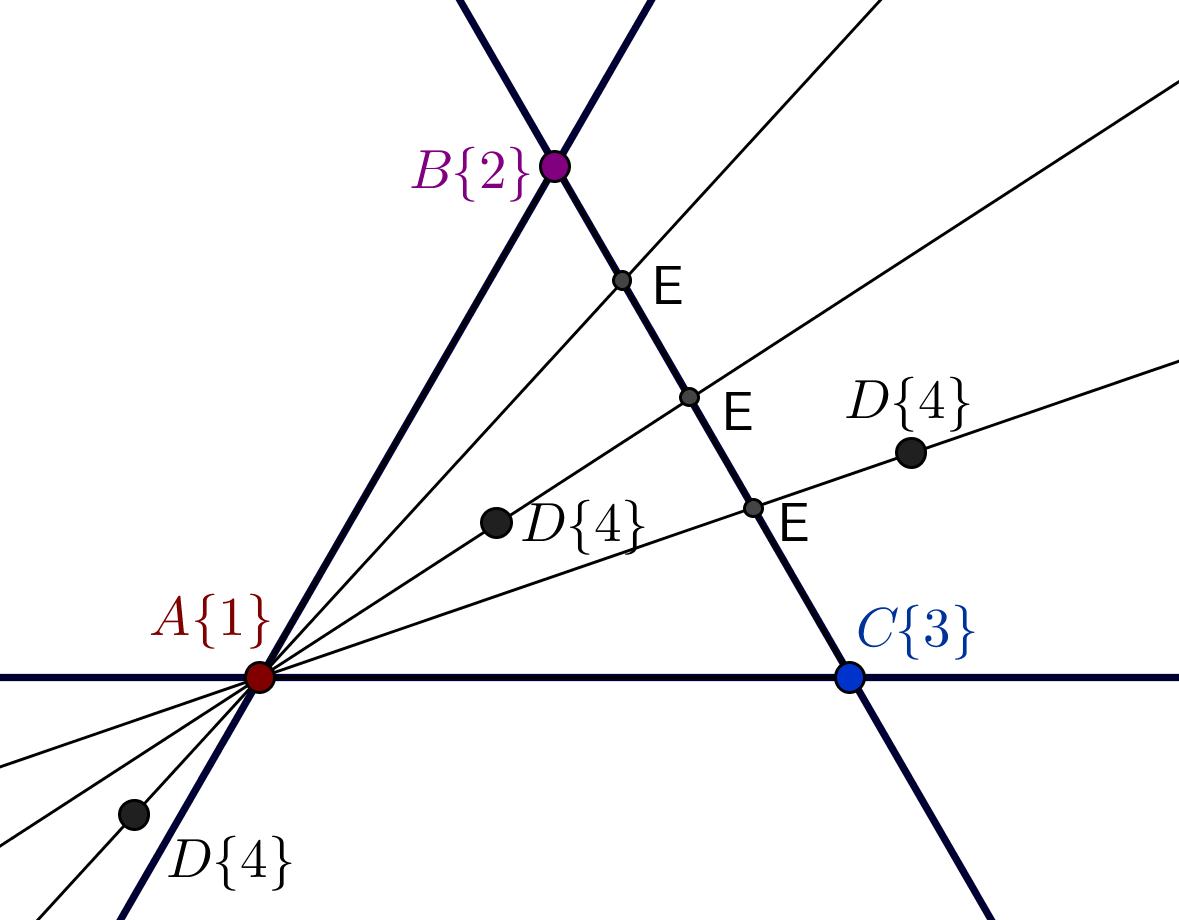
\includegraphics[scale = 0.5]{my_claim1}
				\end{center}
				
				\noindent Прямые $AD$ и $BC$ в~таких случаях не~будут параллельны. Пусть~$E$~– точка пересечения $AD$ и $BC$.
				Тогда с~одной стороны, точка~$E$ должна быть цвета точки~$A$ или точки~$D$, а с~другой~– цвета~$B$ или~$C$. Получаем противоречие. 
		\end{proof}
\end{claim}

\begin{claim}
		Пусть раскраска плоскости такова, что для~любого~$\epsilon > 0$ нельзя выбрать круг радиуса~$\epsilon$,
		покрашенный ровно в~один цвет. Тогда при~такой раскраске для~любого~$\delta > 0$
		можно найти 3 точки разных цветов, попадающие в~круг радиуса~$\delta$. \\
		\begin{proof}
				Зафиксируем~$\delta > 0$. Предположим, что все круги радиуса~$\delta$ покрашены ровно в~2 цвета
				(условие запрещает им быть покрашенными в~один цвет).
				Замостим плоскость кругами радиуса~$\delta$ (с~пересечениями): \\
				\begin{center}
						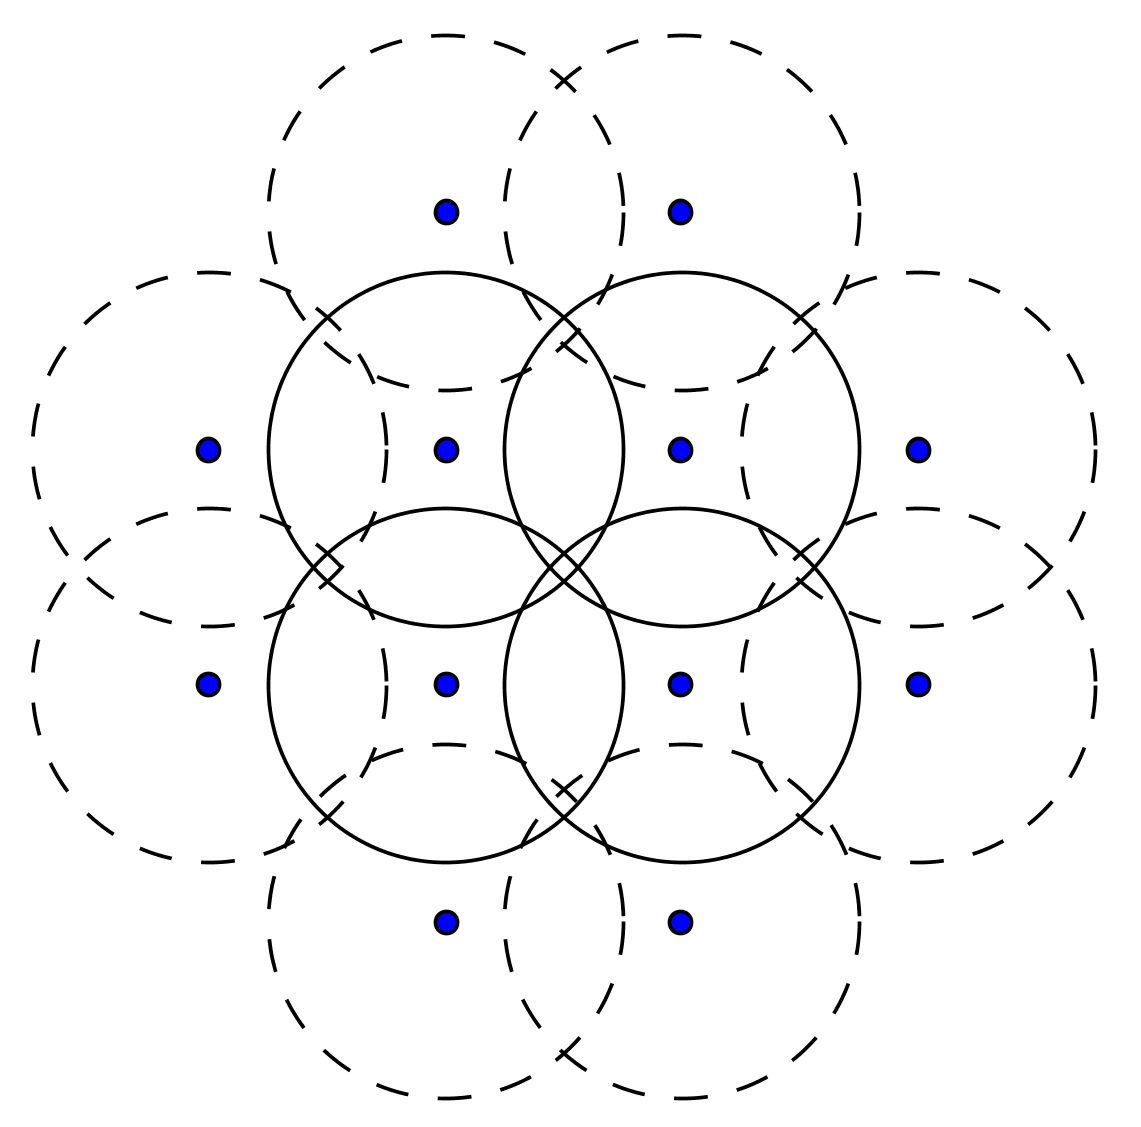
\includegraphics[scale = 0.45]{my_claim2}
				\end{center}
				
				\noindent Выберем некоторый круг, и пусть он раскрашен в~красный и синий цвета.
				Тогда любой «соседний» с~ним круг тоже раскрашен в~красный и синий цвета,
				т.к. их~пересечение содержит круг маленького радиуса, который по~условию не~может быть только одного цвета.
				Итак, цвета в~раскраске «соседних» кругов те~же, что и в~раскраске выбранного круга.
				Таким образом можно «дойти» до~каждой точки плоскости.
				Получаем, что плоскость раскрашена правильно всего в~2 цвета, чего быть не~может.
		\end{proof}
\end{claim}

\begin{remark}
		Существует число~$\delta > 0$ и правильная раскраска плоскости,
		при~которой нельзя указать 4~точки разных цветов, которые можно «накрыть» кругом радиуса~$\delta$. \\
		\begin{proof}
				Рассмотрим раскраску плоскости, которая использовалась для~оценки~$\chi(\mathbb{R}^2) \leq 7$.
				Остается выбрать число~$\delta$ достаточно маленьким. 
		\end{proof}
\end{remark}

\begin{claim}
		Рассмотрим в~пространстве~$\mathbb{R}^3$ равнобедренный треугольник~$ABC$ с~основанием~$AB$ длины~$1$.
		Пусть~$r$~– длина высоты, проведенной к~основанию, и~$r > \frac{1}{2}$.
		Множество, состоящее из~вершин этого треугольника обозначим через~$\Delta$. Имеем
		\begin{equation}
				\pi^3(\Delta) = 3
		\end{equation}
		\begin{proof}
				Зафиксируем~$r$. Покажем сначала, что если в~пространстве найдется окружность~$S_r^1$
				радиуса~$r$, покрашенная хотя~бы в 3~цвета, то утверждение будет доказано.
				Рассмотрим прямую, проходящую через центр~$O$ окружности~$S_r^1$ перпендикулярно плоскости, ее содержащей.
				На~этой прямой отметим точки~$A$ и $B$ на~расстоянии~$\frac{1}{2}$ от~точки~$O$.
				Так как окружность~$S_r^1$ покрашена хотя~бы в 3~цвета,
				то найдется точка~$C \in S_r^1$, цвет которой будет отличен от~двух цветов~$A$ и $B$.
				Значит, удалось обнаружить трехцветное множество~$\Delta$. \\
				\begin{center}
						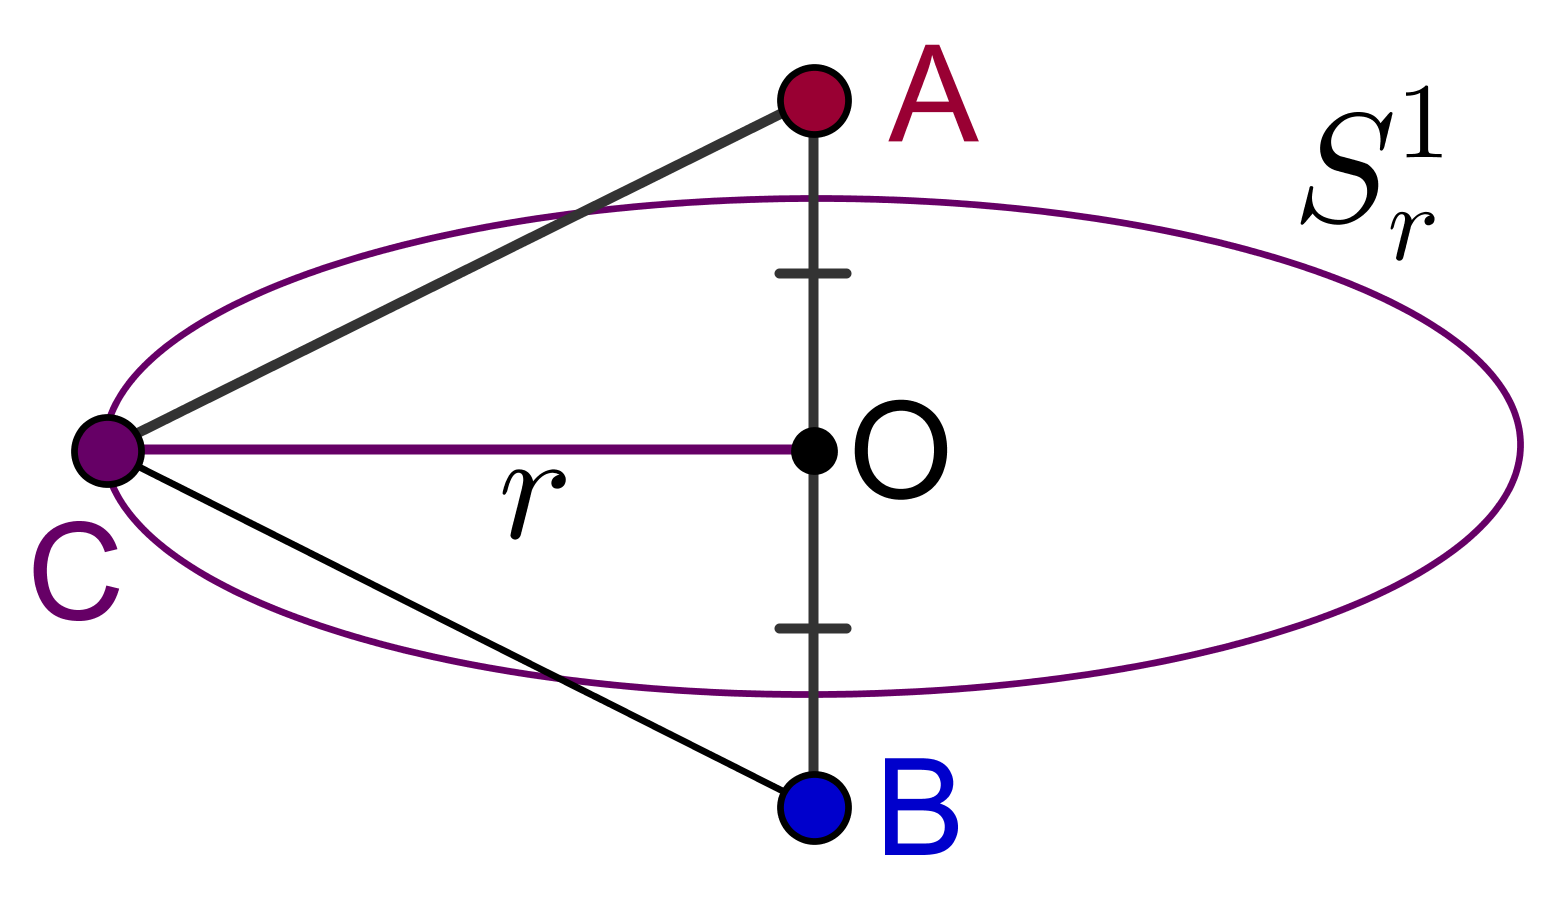
\includegraphics[scale = 0.5]{my_claim3}
				\end{center}
				
				\noindent Остается случай, когда все окружности радиуса~$r$ покрашены в 2~цвета.
				Рассмотрим две точки~$D$ и $E$ на~расстоянии~$2r$ друг от~друга, покрашенные в~разные цвета.
				Такие точки найдутся, потому что в~любом равнобедренном треугольнике с длинами сторон $2r$, $2r$, $1$
				одна из~боковых сторон будет покрашена в~2 разных цвета (используем, что $r > \frac{1}{2}$).
				Все окружности с~диаметром~$DE$ двуцветны по~предположению, а значит и сфера~$S_r^2$,
				являющаяся объединением этих окружностей, также покрашена только в цвета точек~$D$ и $E$.
				Однако тот факт, что двумерная сфера покрашена в 2~цвета, противоречит теореме~Л.~Ловаса:
				
				\begin{theorem}[Л.Ловас 1983 г.]
						При $r > \frac{1}{2}$ имеет место $\chi(S_r^n) \geq n + 1$.
				\end{theorem}
				Для $n = 2$ получаем $\chi(S_r^2) \geq 3$.
				Значит, сфера~$S_r^2$ не~может быть покрашена в 2~цвета, и получено противоречие.
		\end{proof}
\end{claim}

\begin{thebibliography}{4}

\bibitem {Kupavsky2009} \textsc{А.Б. Купавский}:\ \textit{«О поднятии оценки хроматического числа
 $\mathbb{R}^n$ в б\'{о}льшую размер-ность»},  Доклады Российской Академии Наук, \textbf{429:3} (2009), 305 - 308.

\bibitem {Kupavsky2011} \textsc{А.Б. Купавский}:\ \textit{«О раскрасках сфер, вложенных в $\mathbb{R}^n$»},
Матем. сборник, \textbf{202:6} (2011), 83–110.

\bibitem {Raigor2003} \textsc{А.М Райгородский}:\ \textit{Хроматические числа}, МЦНМО, Москва, 2003.

\bibitem {Nechushtan2002} \textsc{O. Nechushtan}:\ \textit{«On the space chromatic number»},
 Discrete Math., \textbf{256} (2002), 499-507.

\end{thebibliography}

\end{document}

\end{document}
